 \documentclass[12pt]{article}

\usepackage[margin=1in]{geometry}
\usepackage{fancyhdr}
\usepackage{setspace}
\pagestyle{fancy}
\usepackage{amsmath, amsthm, amssymb, amsfonts, mathtools, xfrac,mathrsfs}
\usepackage[utf8]{inputenc}
\usepackage[english]{babel}
\usepackage{graphicx,dsfont}
\usepackage{braket, bm}

\everymath{\displaystyle}
\headheight=20pt


\newcommand{\N}{\mathbb{N}}
\newcommand{\Z}{\mathbb{Z}}
\newcommand{\Q}{\mathbb{Q}}
\newcommand{\R}{\mathbb{R}}
\newcommand{\E}{\mathrm{E}}
\newcommand{\Var} {\mathrm{Var}}
\newcommand{\Cov}{\mathrm{Cov}}
\newcommand{\F}{\mathbb{F}}

\DeclareMathOperator{\Tr}{Tr}

\def\mean#1{\left< #1 \right>}
 
\newcommand*\rfrac[2]{{}^{#1}\!/_{#2}}
 
\newenvironment{theorem}[2][Theorem]{\begin{trivlist}
\item[\hskip \labelsep {\bfseries #1}\hskip \labelsep {\bfseries #2}]}{\end{trivlist}}

\newenvironment{problem}[2][Problem]{\begin{trivlist}
\item[\hskip \labelsep {\bfseries #1}\hskip \labelsep {\bfseries #2}]}{\end{trivlist}}

\title{Homework}
\lhead{Math OSM Lab}
\chead{Homework 6 - 8/31/17}
\rhead{Dan Ehrlich}
 
\begin{document}

\begin{problem}{8.1.} We graph the feasible set below. To find the optimizer, plot the objective function over the feasible set and find the maximum point. The optimizer is at $(14/5, 16/5)$ and the objective function has a value of $6/5$. 
\begin{center}
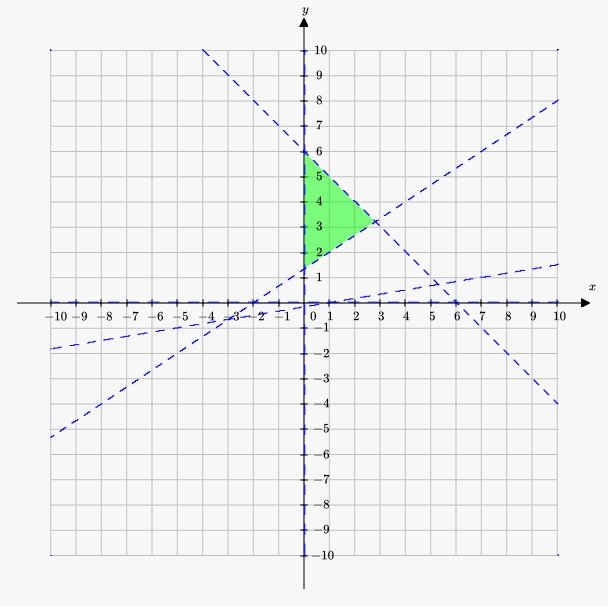
\includegraphics[width=8cm, height=8cm]{prob1.jpeg}
\end{center}
\end{problem}

\begin{problem}{8.2.}\hfill
\begin{itemize}
\item[(i)]We graph the feasible set below. The optimizer is at $(6, 2)$ and the objective function has a value of $20$ at the optimizer. 
\begin{center}
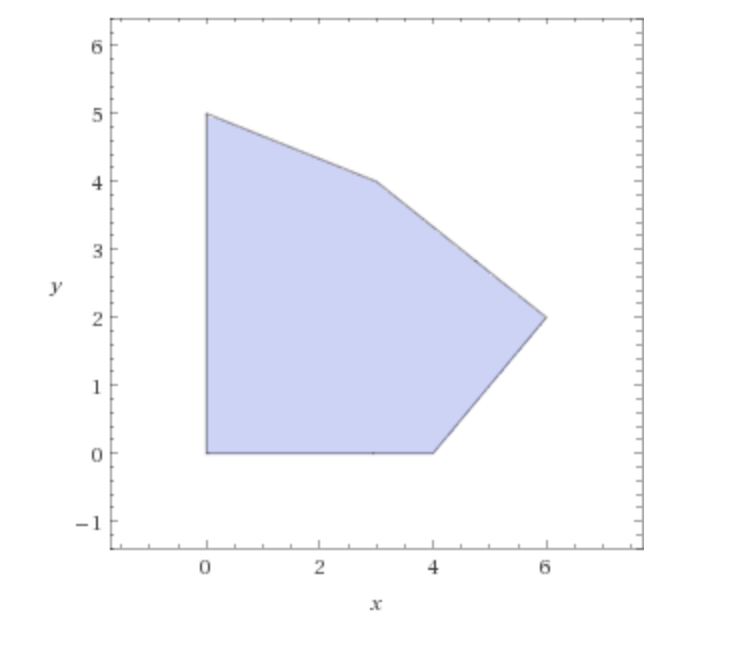
\includegraphics[width=8cm, height=8cm]{prob8i}
\end{center}
\item[(ii)]We graph the feasible set below. The optimizer is at $(15, 12)$ and the objective function has a value of $132$ at the optimizer. 
\begin{center}
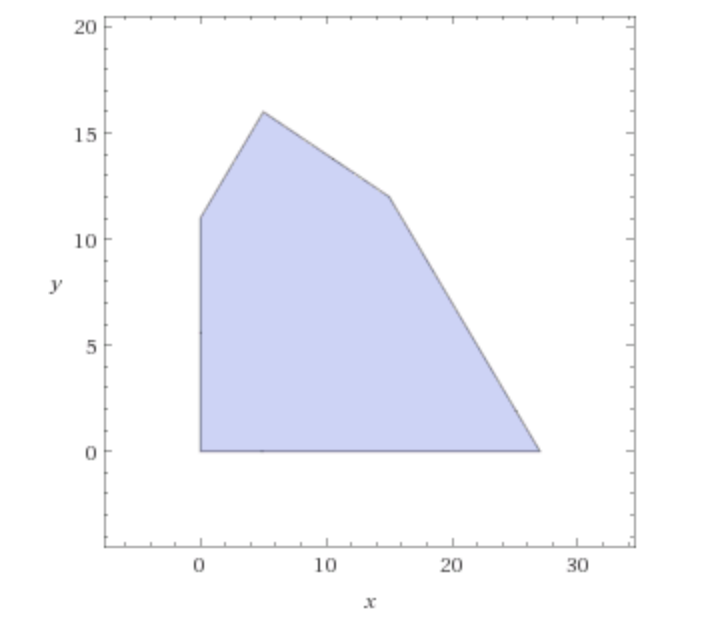
\includegraphics[width=8cm, height=8cm]{prob8ii}
\end{center}
\end{itemize}
\end{problem}

\begin{problem}{8.5.}\hfill
\begin{itemize}
\item[(i)] We use the simplex algorithm to solve the optimization (both by hand and using the Simplex Algorithm we coded for a computation problem set). The result after the first pivot is: $\{2:11 , 3:10, 4:4,0:0, 1:0\}$. After the second pivot the results are, $\{2:3 ,1:2, 0:6, 3:0, 4:0\}$. We see that the results to the optimization are the same as in problem 8.2. 
\item[(ii) ]We use the simplex algorithm to solve the optimization(both by hand and using the Simplex Algorithm we coded for a computation problem set). The result after the first pivot is: $\{2:38, 0:27, 4:36, 3:0, 1:0\}$. After the second pivot the results are, $\{2:14 ,0:15, 1:12, 3:0, 4:0\}$. We see that the results to the optimization are the same as in problem 8.2. 
\end{itemize}
\end{problem}

\begin{problem}{8.7.} \hfill
\begin{itemize}
\item[(i)] We use the simplex algorithm we coded for a computation problem set to solve for the optimizer. The optimizer is at $(3, 4)$ and the objective function has a value of $11$ at the optimizer. 
\item[(ii)] This optimization is unsolvable. The program returns an error. 
\item[(iii)] We use the simplex algorithm we coded for a computation problem set to solve for the optimizer. The optimizer is at $(0, 2)$ and the objective function has a value of $2$ at the optimizer. 
\end{itemize}
\end{problem}

\begin{problem}{8.13.} 
Consider the linear problem 
\begin{align*}
\max \hspace{1cm} & c^Tx &\\
 \text{ s.t } \hspace{1cm}  & Ax \geq 0& \\
 & x \geq 0&
\end{align*}
Let $x = 0$ not be an optimum point. Then by the second assumption there exists a solution $x > 0$ that satisfies the conditions. However, if $x$ satisfies the conditions that $Ax \geq 0$ and $x >0$ then the vector $\lambda x$ where $\lambda > 1$ also satisfies $A\lambda x \geq 0 $ and $\lambda x > 0$. Therefore the problem is unbounded. Now let the problem be bounded. Then by the above proof there does not exist an $x > 0$ that satisfies the conditions. But $x = 0$ satisfies the conditions $Ax \geq 0$ and $x \geq 0$ and therefore is the optimal point. 
\end{problem}

\begin{problem}{8.17.} 
We have that the primal problem can be written as
\begin{align*}
\max \hspace{1cm} & c^Tx &\\
 \text{ s.t } \hspace{1cm}  & Ax \geq b& \\
 & x \geq 0&
\end{align*}
This implies that the dual problem can be written as
\begin{align*}
\min \hspace{1cm} & b^Ty &\\
 \text{ s.t } \hspace{1cm}  & A^Ty \geq c&\\
 & y \geq 0& 
\end{align*}
Then the dual to the dual problem can be written as
\begin{align*}
\min \hspace{1cm} & -c^Tx &\\
 \text{ s.t } \hspace{1cm}  & -Ax \leq -b &\\
 &x \geq 0& 
\end{align*}
which when one removes the negatives is the primal problem.
\end{problem}

\begin{problem}{8.18.} 
We have that the linear problem is
\begin{align*}
\max \hspace{1cm} & x_1 +x_2 &\\
 \text{ s.t } \hspace{1cm}  & 2x_1 + x_2 \leq 3 0& \\
 &x_1 + 3x_2 \leq 5 &\\
 &2x_1 + 3x_2 \leq 4 &\\
 &x_1, x_2 \geq 0
\end{align*}
Then the dual problem is
\begin{align*}
\min \hspace{1cm} & 3y_1 + 5y_2 + 4y_3 &\\
 \text{ s.t } \hspace{1cm}  &  2y_1+y_2+2y_3 \geq 1& \\
 & y_1+3y_2+3y_3 \geq 1& \\
  & y_1,y_2,y_3 \geq 0&
\end{align*}
We solve both using the Simplex Algorithm code and get optimizers of $(1.25, 0.5)$ and $(0.25, 0, 0.25)$ respectively and equal optimal values of 1.75 for both problems. 
\end{problem}

\end{document}

